\documentclass[11pt]{article}
\usepackage[margin=0.85in]{geometry}
\usepackage{amsmath,amssymb,booktabs,longtable,array,hyperref,graphicx}
\newcommand{\R}{\mathbb R}
\newcommand{\F}{\mathcal F}
\newcommand{\U}{\mathcal U}
\newcommand{\X}{\mathcal X}
\newcommand{\cP}{\mathcal P}
\newcommand{\cR}{\mathcal R}
\newcommand{\nn}{\boldsymbol n}
\newcommand{\DD}{\boldsymbol D}
\newcommand{\hh}{\boldsymbol h}
\newcommand{\ssigma}{\boldsymbol\sigma}
\title{C6. Nearest-neighbor qubit chains and the $c$--$d$ conjecture}
\author{Closed-book calculation}
\date{October 27, 2026}
\begin{document}
\maketitle

The conjecture is not settled here for a general nearest-neighbor qubit chain.
There is a proof for the quadratic Jordan--Wigner class using the quasi-free
theorem supplied in the question. The uniform $U(1)$ and zero-field XYZ classes
obey the bound using explicitly stated standard inputs from their exact
solutions. These sets leave a large, precisely specified residual set. Neither
the number of Pauli matrices nor the rank of commuting on-site charges closes
that gap. The numerical calculations below test several points in the residual
set, including short-chain entropy fits exceeding one. They are not a global
exclusion of $c>1$.

No external sources or pre-existing project files were consulted. Statements
marked ``standard input'' are recalled results, not results proved in this
calculation. Numerical identification of a universality class is also kept
separate from proof. All spin matrices below are Pauli matrices, not
$\ssigma/2$, the lattice spacing is one, and $c$ is the usual nonchiral central
charge, with an Ising theory having $c=1/2$.

\section{Parameter space and exact equivalences}

Write
\begin{equation}
 H=\sum_j\left[\ssigma_j^T J\ssigma_{j+1}+\hh\cdot\ssigma_j\right],
 \qquad J=S+A,\quad S^T=S,\quad A_{ab}=\epsilon_{abc}D_c.
 \label{eq:H}
\end{equation}
Thus $D_z$ multiplies $X_jY_{j+1}-Y_jX_{j+1}$. There are twelve real parameters
before removing rotations and scale. A global on-site unitary acts on Pauli
matrices by $R\in SO(3)$ and takes $(S,\DD,\hh)$ to
$(RSR^T,R\DD,R\hh)$. Diagonalizing $S$ gives three eigenvalues and two
three-vectors. Dividing by positive scale gives the generic dimension eight.
The quotient is stratified, not a smooth eight-dimensional manifold everywhere.
All codimensions below mean eight minus the dimension of the indicated stratum
in this quotient.

One can fix, for example,
$\operatorname{tr}S^2+2|\DD|^2+|\hh|^2=1$ and order the eigenvalues of $S$.
Residual proper signed permutations act on the vectors as well as the axes.
At a repeated eigenvalue there remains a continuous basis freedom inside its
eigenspace. The zero Hamiltonian is omitted. A negative rescaling is not an
allowed low-energy equivalence: antiferromagnetic and ferromagnetic Heisenberg
chains already show why.

An additive constant and a bond term $B\otimes1-1\otimes B$ do not affect the
periodic problem. Positive rescaling changes velocities but not central charge.
Translations relabel the same Hamiltonian. Spatial reflection takes
\begin{equation}
 (S,\DD,\hh)\longmapsto(S,-\DD,\hh),
\end{equation}
and spin time reversal takes
\begin{equation}
 (S,\DD,\hh)\longmapsto(S,\DD,-\hh).
\end{equation}
Both are isospectral equivalences between parameter points. They are symmetries
of an individual point only when that point satisfies the corresponding
invariance condition. These two sign changes, together with residual proper
axis sign changes, allow $D_x,D_y,D_z\geq0$ in a generic ordered principal frame,
and then one overall sign choice for $\hh$. Zeros require the usual separate
choice of a representative. These discrete identifications do not change
dimensions.

For completeness, an improper orthogonal matrix $O$ is implemented on Pauli
operators by an antiunitary. Its action is
\begin{equation}
 S\mapsto OSO^T,\qquad \DD\mapsto (\det O)O\DD=-O\DD,
 \qquad\hh\mapsto O\hh. \label{eq:anti}
\end{equation}
The axial-vector sign in this formula is important.

\paragraph{Staggered rotations.}
Let $R=2\nn\nn^T-I$ be a $\pi$ rotation and rotate every other site. The two bond
matrices become $JR$ and $RJ$ in a suitable convention. A uniform field stays
uniform only if $R\hh=\hh$. Consequently the transformed chain is again of
the stated one-site-uniform form if and only if
\begin{equation}
 [J,R]=0,\qquad R\hh=\hh.
 \label{eq:stagger}
\end{equation}
For a $\pi$ rotation, these conditions are
$S\nn\parallel\nn$, $\DD\parallel\nn$, and $\hh\parallel\nn$.
With $\nn=\hat z$ and diagonal $S$ this gives
\begin{equation}
 (J_x,J_y,J_z,D_z,h_z)\mapsto(-J_x,-J_y,J_z,-D_z,h_z).
\end{equation}
Thus it does not give unrestricted independent sign flips for a generic bond.
On even rings it is a product unitary. On odd rings a seam is left; the bulk
central charge is unchanged. In the XYZ class, rotations about any principal
axis are permitted, so any pair of coupling signs can be flipped.

There is a useful exhaustive algebraic test for arbitrary site-dependent
rotations. Given $R_j\in SO(3)$, the transformed chain is uniform precisely when
there are $J',\hh'$ with
\begin{equation}
 R_j^TJR_{j+1}=J',\qquad R_j^T\hh=\hh'\quad\hbox{for every }j.
 \label{eq:gauge}
\end{equation}
For period two this reduces to
$R_e^TJR_o=R_o^TJR_e$ and $R_e^T\hh=R_o^T\hh$.
These tests include exceptional singular bonds without assuming that every
staggered transformation works. Product rotations preserve bipartite entropy
exactly. A fixed-period transformation can change the representation of
translation, but cannot change the bulk central charge.

\paragraph{Spiral rotations.}
A uniform $U(1)$ bond has
\begin{equation}
 S=a(I-\nn\nn^T)+b\nn\nn^T,\qquad
 \DD=d\nn,\qquad\hh=g\nn. \label{eq:U1}
\end{equation}
Take $\nn=\hat z$. The coefficient of
$\sigma_j^-\sigma_{j+1}^+$ is $2(a-id)$, with its conjugate for the reverse
process. A rotation whose angle advances by a constant $\phi$ on each site
removes the phase of $a-id$. Hence the bulk Hamiltonian is equivalent to
\begin{equation}
 H_{\rm XXZ}=\sum_j\left[r(X_jX_{j+1}+Y_jY_{j+1})+
 bZ_jZ_{j+1}+gZ_j\right],\qquad r=\sqrt{a^2+d^2}.
 \label{eq:xxz}
\end{equation}
The ring acquires a twist $L\phi$ modulo $2\pi$. The equality follows directly
by multiplying each raising/lowering operator by its rotation phase. It is
not valid for a transverse field or unequal transverse symmetric couplings:
these acquire spatial phases. A twist selects different zero-mode sectors and
can change the $1/L$ ground-state coefficient along a sequence of sizes, but
not the bulk central charge. Thus the three-dimensional uniform $U(1)$ stratum
has a two-parameter bulk representative $(b/r,g/r)$ when $r>0$.

\paragraph{Jordan--Wigner and Kramers--Wannier.}
Jordan--Wigner is an exact mapping with fermion-parity-dependent boundary
conditions. Nearest-neighbor $XX,YY,XY,YX$ and an axial field are quadratic.
$ZZ$ is a density interaction; transverse fields and mixed axial/transverse
bonds produce strings. The quadratic criterion is proved in Section 3.

For the $Z_2$-symmetric chain, define dual spins by
\begin{equation}
 \tau_j^z=X_jX_{j+1},\qquad Z_j=\tau_{j-1}^x\tau_j^x.
\end{equation}
Direct multiplication gives
\begin{align}
 X_jX_{j+1}&=\tau_j^z,\\
 Y_jY_{j+1}&=-\tau_{j-1}^x\tau_j^z\tau_{j+1}^x,\\
 Z_jZ_{j+1}&=\tau_{j-1}^x\tau_{j+1}^x,\\
 \sum_j(X_jY_{j+1}-Y_jX_{j+1})
 &=\sum_j(\tau_j^x\tau_{j+1}^y-\tau_j^y\tau_{j+1}^x).
 \label{eq:KW}
\end{align}
For example, $Y_jY_{j+1}=-X_jX_{j+1}Z_jZ_{j+1}$ proves the second line.
The axial field becomes a nearest-neighbor $\tau^x\tau^x$ coupling. Thus this
KW transformation stays nearest-neighbor and two-body for
$J_y=J_z=0$ in the chosen axes, including an axial DM term. For general XYZ
couplings it generates a three-site cluster term and/or a next-nearest-neighbor
coupling. Generic transverse spin operators become dual strings. Periodic KW
duality requires the constraint and twisted sectors; it is not a unitary
identification of two unconstrained periodic Hilbert spaces. It preserves the
bulk stress tensor and central charge after that bookkeeping.

Particle-hole transformations and spin-axis changes are contained in these
spin rotations and Jordan--Wigner descriptions. The zero-field XY chain can
also be rearranged into two Majorana/Ising chains; two critical Ising sectors
give total $c=1$. XYZ's eight-vertex description supplies integrability, not a
generic integrability-preserving field perturbation. Clifford conjugations,
for example a layer of controlled-$Z$ gates taking $X_j$ to
$Z_{j-1}X_jZ_{j+1}$, generally increase range. They do not provide a general
nearest-neighbor reduction. Equations \eqref{eq:gauge} and \eqref{eq:KW} state
the range restrictions used here. No exhaustive theorem classifying every
possible nonlocal duality is assumed or claimed.

\section{Symmetry classification and codimensions}

Here ``internal symmetry'' means the same on-site operation on every site.
Translation is always present. Spatial and staggered symmetries are recorded
separately, since otherwise the proposed categories ``none'' and ``only
antiunitary'' are ambiguous.

The complete tests for uniform on-site symmetry are
\begin{align}
 G_u&=\{R\in SO(3):RSR^T=S,\ R\DD=\DD,\ R\hh=\hh\},\label{eq:Gu}\\
 G_a&=\{O\in O(3):\det O=-1,\ OSO^T=S,\ O\DD=-\DD,\ O\hh=\hh\}.
 \label{eq:Ga}
\end{align}
They apply also at repeated eigenvalues. If $S$ has three different
eigenvalues, its proper stabilizer is the identity and the three principal-axis
$\pi$ rotations. A nonidentity one fixes only its axis. It survives if and
only if both vectors lie on that axis. Two different surviving $\pi$ rotations
force both vectors to vanish, and then all three survive. If a continuous
rotation survives, $S$ must be scalar in its transverse plane and both vectors
must lie on its axis. In fact a single proper rotation with angle different
from zero and $\pi$ already forces these conditions, and hence the entire
axial $SO(2)$. This excludes additional finite rotation groups without a
continuous enhancement. The complete classification of $G_u$ is therefore:
\begin{itemize}
\item $C_2$: $S\nn\parallel\nn$, both vectors parallel to $\nn$, at least one
  nonzero, and the transverse restriction of $S$ not scalar.
\item $D_2\simeq Z_2\times Z_2$: both vectors zero and $S$ has distinct eigenvalues.
\item $SO(2)$: equation \eqref{eq:U1} with at least one vector nonzero.
\item $O(2)$ embedded in $SO(3)$: both vectors zero and exactly two eigenvalues
  equal. This includes the transverse $\pi$ rotations as well as axial rotations.
\item $SO(3)$: both vectors zero and $S$ scalar.
\item The trivial group in all remaining cases.
\end{itemize}
The projective spin-$1/2$ implementation of $D_2$ is understood. The rotations
commute as operations on Pauli vectors; their on-site unitary representatives
need not commute as matrices.

If $G_u$ is trivial but an antiunitary survives, there can be only one
improper Pauli action, since the product of two would be a nontrivial proper
action. Its square must be the identity. An improper orthogonal involution
in three dimensions is either $-I$ or a plane reflection. Therefore the
antiunitary-only possibilities are exactly
\begin{align}
 &\hh=0\quad\hbox{(time reversal)},\label{eq:Tclass}\\
 &S\nn\parallel\nn,\quad \DD\parallel\nn,\quad \hh\perp\nn
 \quad\hbox{(reflection of the spin component along }\nn\hbox{)},
 \label{eq:Kclass}
\end{align}
with the points having nontrivial $G_u$ removed. The plane-reflection
antiunitary squares to $+1$ on a single spin, whereas time reversal squares to
$-1$. These conditions, not just the generic diagonal-frame description,
cover degeneracies of $S$.

\begin{center}
\small
\begin{tabular}{p{0.29\linewidth}c c p{0.40\linewidth}}
\toprule
Class & Dimension & Codimension & Status of $c\leq1$\\
\midrule
Quadratic JW locus $\F$ & 3 & 5 & Proved using the given quasi-free theorem.\\
Uniform $U(1)$ locus $\U$ & 3 & 5 & Standard XXZ input; includes its enhanced strata.\\
XYZ, $\X=\{\DD=\hh=0\}$ & 2 & 6 & Standard XYZ gap classification and XXZ input.\\
Exactly one unitary $Z_2$ & 4 & 4 & Open off the controlled subloci. Targeted ED below.\\
Only antiunitary, time-reversal branch & 5 & 3 & Open.\\
Only antiunitary, plane-reflection branch & 5 & 3 & Open.\\
No nontrivial uniform internal symmetry & 8 & 0 & Open. Targeted ED below.\\
Enhanced $O(2)$, zero vectors & 1 & 7 & Contained in XXZ/XYZ.\\
Enhanced $SO(3)$ & 0 & 8 & Heisenberg only; standard AF result or nonconformal FM.\\
\bottomrule
\end{tabular}
\end{center}
Rows overlap where stated. ``Only antiunitary'' and ``no symmetry'' exclude
nontrivial uniform unitary symmetries. Dimensions are maximal dimensions of
the named strata; further degeneracies can have smaller dimensions. They are
not codimensions of criticality inside a class.

To check the counting in a principal frame, the unrestricted data are
$3+3+3-1=8$. A surviving principal-axis $Z_2$ leaves $3+1+1-1=4$;
$D_2$ leaves $3-1=2$. Time reversal leaves $3+3-1=5$ and the reflection branch
leaves $3+1+2-1=5$. Uniform $U(1)$ leaves $2+1+1-1=3$. The free locus removes
one axial eigenvalue from the $Z_2$ family, giving $2+1+1-1=3$.
The enhanced dimensions use the larger stabilizer, rather than subtracting a
three-dimensional rotation orbit at every point.

Pure spatial reflection is a symmetry when $\DD=0$. Reflection combined with
a proper spin rotation obeys
$RSR^T=S$, $R\DD=-\DD$, $R\hh=\hh$.
Reflection combined with an antiunitary obeys
$OSO^T=S$, $O\DD=\DD$, $O\hh=\hh$, $\det O=-1$.
For instance, the axial $Z_2$ family with both $D_z$ and $h_z$ nonzero has no
uniform internal antiunitary generically, but does have such a combined
spatial antiunitary. Calling it entirely antiunitary-free would be incorrect.

There are also staggered continuous symmetries. For example,
\begin{equation}
 H=\sum_j[a(X_jX_{j+1}-Y_jY_{j+1})+bZ_jZ_{j+1}+gZ_j]
\end{equation}
commutes with $\sum_j(-1)^jZ_j$ on an even ring. A staggered $\pi$ rotation
about $x$ maps it to XXZ with a staggered longitudinal field. For $g\ne0$ this
is not the uniform-field Bethe-ansatz class. Generically this is a
codimension-six sublocus of the uniform-$Z_2$ row and remains uncontrolled
here when $b\ne0$. More general site-dependent symmetries are tested by
\eqref{eq:gauge}; they should not be confused with uniform internal ones.

\section{Controlled classes}

Define the following rotation-invariant loci in $\cP$:
\begin{align}
 \F&=\{\exists\nn,\ |\nn|=1:\ S\nn=0,\ \DD\parallel\nn,
                  \ \hh\parallel\nn\},\label{eq:F}\\
 \U&=\{\exists\nn:\ S=a(I-\nn\nn^T)+b\nn\nn^T,
                  \ \DD\parallel\nn,\ \hh\parallel\nn\},\\
 \X&=\{\DD=\hh=0\}.
\end{align}
The zero vector is considered parallel to every axis.

\subsection{Quadratic class: a proof}

Choose $\nn=\hat z$ and diagonalize the transverse symmetric block by a
rotation about $z$. The Hamiltonian on $\F$ is
\begin{equation}
 H=\sum_j[J_xX_jX_{j+1}+J_yY_jY_{j+1}
       +D(X_jY_{j+1}-Y_jX_{j+1})+gZ_j].
\end{equation}
With $c_j=(\prod_{l<j}Z_l)\sigma_j^+$ and $n_j=c_j^\dagger c_j$, one has
$Z_j=1-2n_j$. Multiplication gives
\begin{align}
 H=\sum_j\{& (J_x+J_y-2iD)c_j^\dagger c_{j+1}
          +(J_x+J_y+2iD)c_{j+1}^\dagger c_j\\
 &+(J_x-J_y)(c_j^\dagger c_{j+1}^\dagger+c_{j+1}c_j)
       +g(1-2n_j)\}. \label{eq:JW}
\end{align}
The ring boundary condition is fixed by fermion parity. There are two real
Majoranas per physical site and only nearest-neighbor quadratic couplings.
The theorem supplied in the question therefore gives
\begin{equation}
 c_T\leq\frac{\operatorname{rank} A(1)}2\leq\frac22=1.
\end{equation}
Here $A(1)$ denotes the intersite Majorana matrix in that theorem, not the
antisymmetric spin coupling $A$ in \eqref{eq:H}. This is a proof conditional
only on the explicitly supplied theorem and the conformal hypothesis.

Conversely, for ordinary JW about a fixed axis the independent Pauli strings
show that an axial $ZZ$ bond is quartic, axial/transverse bonds give odd
strings, and transverse on-site fields give strings. Such terms cannot
cancel the even quadratic strings in a uniform bulk sum. Thus they must
vanish to obtain a purely quadratic bulk Hamiltonian. In coordinate-free
form the bond must have a common left and right null axis,
$J\nn=J^T\nn=0$, and $\hh\parallel\nn$. Adding and subtracting the two null
conditions gives $S\nn=0$ and $A\nn=0$, equivalent to \eqref{eq:F}.
If different local JW axes are allowed, every site axis must lie in both
$\ker J$ and $\ker J^T$ for a uniform bond, and align with the uniform field
when it is nonzero. Hence this local-axis generalization does not enlarge
the quadratic locus.

For a useful direct check, the bulk BdG eigenvalues can be written
\begin{equation}
 \lambda_\pm(k)=4D\sin k\pm
 2\sqrt{[(J_x+J_y)\cos k-g]^2+(J_x-J_y)^2\sin^2 k},
 \label{eq:disp}
\end{equation}
up to reversing $k$ by convention. A single massless Majorana gives $c=1/2$;
two give total $c=1$. Coincident zeros do not allow $c=3/2$ by the rank bound.
When $g=J_x+J_y$ and $2|D|=|J_x-J_y|\ne0$, the tilt cancels a linear
velocity at $k=0$. Generically the remaining branch starts cubically,
since both the tilt and pairing are odd in $k$ and the normal mass term starts
at $k^2$. This is a nonconformal endpoint, not an additional Ising sector
coexisting with a boson. Other multiple-zero limits must likewise be checked
for nonzero velocities before assigning a CFT central charge.

\subsection{Uniform $U(1)$: reduction and stated Bethe-ansatz input}

Equation \eqref{eq:xxz} proves the reduction to XXZ in a field with a twist.
For $r>0$ set $\Delta=b/r$; in conventional spin-$1/2$ notation the exchange
is $4r$ and the longitudinal magnetic field is $-2g$.

The standard input used here is the exhaustive zero-temperature ground-state
and low-energy solution of the spin-$1/2$ XXZ chain in a uniform longitudinal
field: every conformal gapless phase has one filled Bethe sea with two edges,
one dressed charge, and one oscillator tower at each chirality. There is no
additional independent massless string sea in the ground state. Its free
energy and ground-state Casimir term are
\begin{equation}
 f(T)=e_\infty-\frac{\pi T^2}{6v}+o(T^2),\qquad
 E_0(L)=Le_\infty-\frac{\pi v}{6L}+o(L^{-1})
 \label{eq:BAc}
\end{equation}
in the untwisted vacuum sector. At nonzero twists the zero-mode energy must
be added. These statements, including exhaustiveness of the massless modes,
are the standard finite-size Bethe-ansatz/CFT input, not an assumption that
follows from $U(1)$ symmetry alone.

To see the mechanism, write the Bethe equations as
$Lp(\lambda_j)=2\pi I_j+\sum_l\theta(\lambda_j-\lambda_l)$.
For a single interval $[-B,B]$, differentiating the counting function yields
\begin{equation}
 \rho+K*\rho=p'/(2\pi),\qquad K=\theta'/(2\pi),
 \qquad v=\frac{\varepsilon'(B)}{2\pi\rho(B)}.
\end{equation}
Here the sign convention for $\theta$ fixes the corresponding sign in $K$.
The dressed energy obeys its linear dressing equation with
$\varepsilon(\pm B)=0$, and the dressed charge solves $Z+K*Z=1$ on the same
interval. Independent changes of the two Fermi edges give one charge and
one winding zero mode. Particle-hole rearrangements at each edge give
integer oscillator levels with generating function
$\prod_{n\ge1}(1-q^n)^{-1}$ per chirality. Thus the finite-size spectrum has
the Gaussian form
\begin{equation}
 E-E_0=\frac{2\pi v}{L}\left[
 \frac{(\delta N)^2}{4Z(B)^2}+Z(B)^2D_w^2+N_R+N_L\right]+o(L^{-1}),
\end{equation}
with selection rules and a shift of $D_w$ at a twist. One oscillator character
has chiral Casimir $-1/24$, giving \eqref{eq:BAc} and $c=1$.
This explains how the stated exact-solution input implies the bound. It does
not independently prove Bethe completeness or the finite-size asymptotics.

For $-1<\Delta\le1$ the unsaturated critical region is this single-boson
liquid, including the antiferromagnetic $\Delta=1$, zero-field point with
logarithmic corrections. For $\Delta>1$ there is a gapped low-field Neel
plateau and a one-boson region between its lower critical field and saturation.
The plateau edge and saturation edge have quadratic onset, not a new
relativistic sector. For $\Delta<-1$ there are polarized/gapped phases and
zero-field coexistence, rather than an extra conformal liquid. The
$\Delta=-1$, zero-field endpoint is equivalent to the isotropic ferromagnet
and has quadratic magnons. When $r=0$, the chain is classical Ising in a
longitudinal field; its level crossings or extensive degeneracies are not
unitary conformal spectra with nonzero velocity.

As a normalization check, a flipped spin above the fully polarized state has
minimum energy $2|g|-4b-4r$, so for $\Delta>-1$ the saturation field is
$|g_{\rm sat}|=2r(1+\Delta)$, consistent with a quadratic minimum there.

Some thermodynamic parts of this solution admit rigorous formulations, but
no self-contained proof of the full CFT identification for all fields and
anisotropies is supplied here. Accordingly the table labels this row
``standard input'', not an unconditional mathematical proof developed in
this note. With that input there is no Ising-times-boson point of $c=3/2$ in
the uniform $U(1)$ class.

\subsection{XYZ and enhanced $SU(2)$}

For $\DD=\hh=0$, the staggered sign flips and axis permutations reduce the
couplings to
\begin{equation}
 a\ge b\ge |c|,\qquad a,b\ge0.
\end{equation}
The standard XYZ/eight-vertex ground-state gap classification used here is:
for $a>b$ the bulk has a nonzero excitation gap above its possible broken
symmetry ground-state multiplet. The conformal boundary is
\begin{equation}
 a=b>0,\qquad -a<c\le a.
\end{equation}
It is the XXZ critical line with $c_{\rm CFT}=1$, including the
antiferromagnetic endpoint. The other endpoint $c=-a$ is the ferromagnetic
quadratic-dispersion point after a staggered rotation. The all-zero point has
no conformal dynamics. The exhaustive gap classification is an input from
the XYZ solution; it is not derived by elementary symmetry arguments here.
Once it is supplied, the previous XXZ argument proves the claimed implication.
There is no additional $c>1$ multicritical point in this classification.

There is a separate elementary restriction on exact microscopic $SU(2)$.
Since $\tfrac12\otimes\tfrac12=0\oplus1$ with multiplicity one, its two-site
commutant is spanned by the identity and swap. Therefore an invariant bond
is a constant plus $J\ssigma_j\cdot\ssigma_{j+1}$, with zero field and DM
vector. The antiferromagnet is $SU(2)_1$ by the standard Heisenberg solution.
For $J<0$ a one-magnon state has
$E(k)-E_0=4|J|(1-\cos k)$, so its small-$k$ dispersion is quadratic.
There is no exact-$SU(2)$ nearest-neighbor qubit parameter available to realize
$SU(2)_k$ with $k>1$. This statement does not prohibit an emergent $SU(2)_k$
at a point whose microscopic symmetry is smaller.

\subsection{What further elementary arguments do and do not prove}

For two traceless on-site Hermitian charges,
\begin{equation}
 [\boldsymbol a\cdot\ssigma,\boldsymbol b\cdot\ssigma]
 =2i(\boldsymbol a\mathbin{\times}\boldsymbol b)\cdot\ssigma.
\end{equation}
Commutativity implies that the two vectors are parallel. Thus there is at
most one independent commuting on-site charge modulo the identity. This is
a proof about microscopic charges, not about central charge. A boson times
an Ising CFT has only one required $U(1)$ and has $c=3/2$. Three Ising CFTs
need no continuous symmetry at all. Emergent charges can be non-on-site or
have no microscopic exact conservation law. No upper bound on $c$ follows
from this rank argument without an additional, unproved premise.

Classical commuting longitudinal bonds have no dispersing conformal modes.
For a Hamiltonian that is actually frustration-free, the gapless
nonconformal exclusion supplied in the question can also be used. A
factorized ground state alone does not establish frustration-freeness in the
given bond decomposition, and frustration-freeness cannot be assumed from
a suggestive point in a phase diagram. These observations eliminate some
points, not the residual interacting critical set.

\section{The residual set and the missing argument}

The precise algebraic residual set of this analysis is
\begin{equation}
 \boxed{\cR=\cP\setminus(\F\cup\U\cup\X).} \label{eq:residual}
\end{equation}
The task remaining is to establish or refute $c\le1$ for conformal critical
points in $\cR$. Proven nonconformal points can of course be discarded
individually. The specified global, staggered, and spiral transformations
and the nearest-neighbor KW subcase do not supply a new generic controlled
stratum outside this union. Equation \eqref{eq:residual} is the complement
of the loci controlled here, not a claim that no further isolated exact
solutions or unidentified dualities exist.

In the single-$Z_2$ frame, the uncontrolled parameters are
\begin{equation}
 (J_x,J_y,J_z,D_z,h_z),\qquad
 J_z\ne0,\quad J_x\ne J_y,\quad (D_z,h_z)\ne(0,0),
\end{equation}
with the axis transverse block nonscalar and with positive scale divided
out. The coordinate-free definitions cover accidental degeneracies without
choosing a misleading principal frame. All genuinely antiunitary-only and
internally symmetry-free points lie outside the three controlled loci.

In the single-$Z_2$ family, JW adds to \eqref{eq:JW} the term
\begin{equation}
 J_z\sum_j(1-2n_j)(1-2n_{j+1}).
\end{equation}
This is a nearest-neighbor interacting Kitaev chain with complex hopping,
real pairing, a chemical potential, and density interaction. The free
determinant-root proof is no longer available. In particular the exact
interacting self-energy need not be a degree-one Laurent polynomial.
Mixed axial/transverse spin terms and transverse fields in the other
residual strata remove even this local even-fermion description.

A possible Ising-times-boson point would require a massless neutral Majorana
sector as well as a compact boson, with nonzero velocities and all allowed
relevant couplings tuned away or forbidden. In a $Z_2$-symmetric realization
the Ising magnetic operator may be forbidden, but the Ising energy operator
and allowed boson vertex operators still have to be controlled. Without
$Z_2$, the Ising magnetic perturbation must also be tuned. Couplings such as
an Ising energy density times a boson current are marginal by naive scaling;
other products can be relevant depending on the radius and translation
quantum numbers. These observations identify tuning conditions, not an
impossibility theorem. Eight microscopic parameters do not rule out such
fine tuning by dimension counting.

Nor does $c>1$ logically require a product of two independent CFTs or any
emergent $U(1)$: an interacting irreducible $c>1$ theory is another possibility.
One lattice Pauli operator can contain several continuum primaries at
different momenta, and multi-site operators and strings supply further
fields. Counting three Pauli matrices is not a count of continuum sectors.
The supplied next-nearest-neighbor example, two decoupled Heisenberg
sublattices with total $c=2$, already disproves an upper-bound argument based
only on that local operator count. A successful argument must use the strict
nearest-neighbor restriction in a substantive way.

LSM and anomaly constraints can obstruct a unique symmetric gapped state
and, for the supplied $D_2$ anomaly, impose a lower bound on $c$. They do not
give the missing upper bound. A single unitary $Z_2$ has no analogous
spin-half projective obstruction. Time-reversal Kramers structure can impose
an LSM obstruction, but still does not establish $c\le1$. In a symmetry-free
chain there is no relevant microscopic internal anomaly to use. Anomaly
matching does not generally exclude extra neutral sectors.

The $c$-theorem also cannot start from an assumed free-qubit ultraviolet CFT:
the lattice does not come with such a relativistic fixed point. A flow from
a specified $c=1$ ultraviolet theory would be an extra assumption. The
supplied entropy and thermodynamic obstructions explain why a local Hilbert
space bound cannot be substituted for that assumption.

\section{Numerical method and results}

The reproducible code is \texttt{c6.py}; raw records are in
\texttt{c6\_results.jsonl}. It uses NumPy, SciPy, and Numba on one BLAS thread
per process. No cluster-scale computation was attempted. The largest chains
have $L=22$, and the entire calculation stayed below the requested hour.

For each binary spin configuration $r$, let $p_r$ be its translation orbit
length. In momentum $k=2\pi m/L$, an allowed normalized orbit vector is
\begin{equation}
 |r;k\rangle=p_r^{-1/2}\sum_{t=0}^{p_r-1}e^{-ikt}T^t|r\rangle,
 \qquad mp_r=0\pmod L.
\end{equation}
If a local term sends representative $r$ to $s=T^u r'$, its contribution to
the block matrix is the computational-basis amplitude times
$\sqrt{p_r/p_{r'}}e^{iku}$. This follows by projecting the translation sum
and accounts for shorter orbits. Parity $\prod_jZ_j$ is used only when it is
an exact symmetry. Sparse Hermitian blocks are diagonalized with Lanczos/
ARPACK; the eigenvector residuals are recorded. Ground-state vectors are
expanded back to the spin basis for reduced density matrices.

The implementation was checked against an independently constructed dense
Kronecker-product Hamiltonian for a fully general random real $J$ and field
at $L=6$, comparing all momenta and also the full spectra in the parity
example. An initial expansion check exposed single-precision square roots
of integer orbit lengths in Numba. Casting those lengths to double fixed
the issue. All results used below have \texttt{code\_version=2}; earlier
exploratory records are retained but are not used for reported fits.
After correction the full-spectrum error was $2.14\times10^{-14}$,
Hermiticity error $9.54\times10^{-15}$, and the intertwining error between
the dense and orbit Hamiltonians $3.84\times10^{-14}$. The parity spectrum
error was $9.77\times10^{-15}$. The critical Ising ground-state check against
$E_0=-2/\sin[\pi/(2L)]$ gave error $5.33\times10^{-15}$.

For a conformal ground state on a ring the entropy test is
\begin{equation}
 S_L(\ell)=\frac{c_T}{3}\log\left[\frac L\pi
 \sin\frac{\pi\ell}L\right]+s_0+\cdots.
\end{equation}
The reported $c_{\rm chord}$ is three times the slope using integer cuts
$\max(3,\lfloor L/4\rfloor)\le\ell\le L/2$. It is a finite-size estimator,
not a central charge by definition. A separate size-growth estimator is
\begin{equation}
 c_{\rm step}(L,L')=
 3\frac{S_{L'}(L'/2)-S_L(L/2)}{\log(L'/L)}.
\end{equation}
For energies and towers, allowing unequal chiral velocities gives
\begin{align}
 E_0(L)&=Le_\infty-\frac{\pi}{12L}
 \sum_a c_a(v_{a,R}+v_{a,L})+\hbox{zero-mode shifts}+\cdots,\\
 E_n-E_0&=\frac{2\pi}L\sum_a
 [v_{a,R}(h_a+N_{a,R})+v_{a,L}(\bar h_a+N_{a,L})]+\cdots.
\end{align}
A single fitted velocity cannot determine total $c$ for multiple sectors.
Moving Fermi momenta and finite-size zero-mode changes must also be retained.

\subsection{Calibrations}

The calibrations were $H_I=-\sum(XX+Z)$ and
$H_{XX}=-\sum(XX+YY)$ at $L=12,16,20,22$. Their velocities are respectively
2 and 4. Both parity sectors and momenta $m=0,\pm1,\pm2,L/2$ were sampled.
The exact/Perron--Frobenius ground-state information places their ground
states in $m=0$. Fit $E_0/L=e_\infty+a/L^2+b/L^4$ and
$S_L(L/2)=s+(c/3)\log L+b_s/L^2$. The results are
\begin{center}
\begin{tabular}{lrrr}
\toprule
Model & $c_{\rm chord}(22)$ & $c$ from energy & $c$ from half-entropy fit\\
\midrule
Critical Ising & 0.500401 & 0.499998 & 0.500002\\
XX & 1.003542 & 0.999939 & 1.000073\\
\bottomrule
\end{tabular}
\end{center}
These fits use the known velocities. In particular, a chord estimate slightly
larger than one already occurs in the proven $c=1$ free chain.

The Ising momentum/parity towers also pass a separate test. Defining
$v_\pm(L)=L[E_{\mathrm{odd},\pm1}-E_{\mathrm{odd},0}]/(2\pi)$, the $L=22$
values are both 1.993210. With their average as velocity, the odd-sector
primary has $x=0.125479$ and the first even $m=0$ excitation has $x=1.002554$,
approaching $1/8$ and 1. The $m=\pm2$ stress-tensor energies divided by
$4\pi v_\pm/L$ are 0.997452. In the XX calibration the $L=22$ oscillator
velocity is 3.986419 and the lowest opposite-parity charge primary has
$x=0.251279$, approaching $1/4$. These are spectral checks, separate from
fitting an entropy slope.

\subsection{An interacting single-$Z_2$ Ising candidate}

The residual family used for the first search was
\begin{equation}
 H(D,g)=\sum_j[-X_jX_{j+1}-0.5Y_jY_{j+1}+0.25Z_jZ_{j+1}
 +D(X_jY_{j+1}-Y_jX_{j+1})-gZ_j]. \label{eq:numeric-family}
\end{equation}
It lies outside $\F\cup\U\cup\X$ for the parameters tested. At $D=0.1$,
crossings of the parity gap scaled by $L$, in the bracket $1.95<g<2.0$, were
\begin{center}
\begin{tabular}{cc}
\toprule
Sizes & Crossing $g$\\
\midrule
12,16 & 1.982399522\\
14,18 & 1.984826813\\
16,20 & 1.986151490\\
18,22 & 1.986922063\\
\bottomrule
\end{tabular}
\end{center}
Fits of the drift to powers two, three, and four of inverse mean size give
intercepts 1.99146, 1.98937, and 1.98833. These are not a controlled error bar.
The follow-up used the fixed approximate field $g=1.9891$ and checked every
momentum and both parities, retaining four levels per block. Its ground state
was even and at $m=0$ for every size tested.

\begin{center}
\begin{tabular}{rrrrrrr}
\toprule
$L$ & $c_{\rm chord}$ & $S(L/2)$ & $v_+$ & $v_-$ & $x_\sigma$ & $x_\varepsilon$\\
\midrule
12 & .510020 & .458659 & .715779 & 1.479631 & .086232 & .841151\\
16 & .509836 & .514185 & .594105 & 1.373599 & .099890 & .887184\\
20 & .506764 & .554475 & .530392 & 1.317193 & .108246 & .918907\\
22 & .506103 & .571229 & .509481 & 1.298546 & .111240 & .930741\\
\bottomrule
\end{tabular}
\end{center}
Here $v_\pm$ use the odd-primary descendants as in the Ising calibration,
and $x_\sigma,x_\varepsilon$ use their average. These identifications are a
test of the Ising hypothesis, not an independent definition of the spectrum.
The velocity asymmetry is permitted by the DM term. The low dimensions move
toward $1/8$ and 1, and the first odd $m=0$ excitation above the odd primary
has dimension difference 2.06168 at $L=22$, moving toward 2. The two stress
ratios are 1.14046 and 1.04887, so the slowly moving branch still has sizable
finite-size corrections.

The ground-energy fit gives $c\bar v=0.408489$. Extrapolating the descendant
velocities with a constant and $L^{-2}$ gives
$(v_+,v_-)=(0.42527,1.22499)$ and $c_E=0.4951$; adding $L^{-4}$ gives
$(0.40480,1.20470)$ and $c_E=0.5076$. The half-entropy fit gives 0.4871,
whereas the $20$--$22$ step gives 0.5273. Taken together the spectra, energies,
and entropies are consistent with one Ising CFT and finite-size corrections.
They do not establish an exact critical field or a theorem about its basin.

A broad initial crossing bracket also returned $g=1.81414$. This was not
accepted as the critical field. The scaled parity gap oscillates in that
region, and at the nearby $g=1.8$ the chord estimate falls from 0.4954 at
$L=12$ to 0.2796 at $L=16$, while the half entropy decreases. A parity-gap
crossing alone is insufficient.

\subsection{Current-carrying candidates and entropy false positives}

The all-momentum screening of \eqref{eq:numeric-family} used
\begin{equation}
 D\in\{.1,.2,.25,.3,.4,.6\},\qquad
 g\in\{1.2,1.6,1.8,1.9,1.98,2.05\}
\end{equation}
at $L=12,16$, giving 72 size-parameter cases. The largest $L=16$ chord fit
was 1.200584 at $(D,g)=(.4,2.05)$. This point and the more interior point
$(.4,1.2)$ were followed through $L=18,20,22$, checking every momentum and
both parities and retaining four levels per block.

\begin{center}
\begin{tabular}{llrrrr}
\toprule
$(D,g)$ & $L$ & $E_0$ & $S(L/2)$ & $c_{\rm chord}$ & $(p,m)$\\
\midrule
$(.4,1.2)$ & 12 & -17.035492 & 1.142558 & 1.108429 & $(0,4)$\\
 & 16 & -22.678625 & 1.224643 & 1.068883 & $(1,5)$\\
 & 18 & -25.454053 & 1.279569 & 1.075040 & $(0,6)$\\
 & 20 & -28.177104 & 1.292537 & 1.070937 & $(0,6)$\\
 & 22 & -30.972338 & 1.332434 & 1.024714 & $(1,14)$\\
\midrule
$(.4,2.05)$ & 12 & -22.295849 & .743864 & 1.150466 & $(1,1)$\\
 & 16 & -29.749676 & .973935 & 1.200584 & $(0,2)$\\
 & 18 & -33.454844 & .981372 & 1.195548 & $(0,2)$\\
 & 20 & -37.148264 & .988348 & 1.200302 & $(0,2)$\\
 & 22 & -40.835751 & .994942 & 1.194807 & $(0,2)$\\
\bottomrule
\end{tabular}
\end{center}
Here parity is $(-1)^p$. For $(.4,1.2)$ the chord estimates decrease toward
one, consistent with a one-boson liquid, but level rearrangements prevent
an accurate simple extrapolation from these sizes. At $(.4,2.05)$ the
$16$--$22$ half-entropy growth gives $c_{\rm step}=0.197897$, in conflict
with the chord value 1.194807. The abrupt $12$--$16$ entropy increase and
changes of momentum/parity are characteristic of the finite-size sector
problem. The numerical data do not support interpreting 1.19 as a measured
central charge.

The momentum spectra show the same difficulty. At $(.4,2.05)$ the smallest
nonzero $L(E-E_0)/(2\pi)$ values for $L=18,20,22$ are 0.177368, 0.214361,
and 0.022291, respectively. The lowest state's relative momentum and parity
also change. Neither two stable conformal towers nor two nonzero limiting
velocities were identified. A Casimir fit assigning these changing
zero-mode energies to a single velocity would be unjustified. This does not
prove that the thermodynamic phase is nonconformal, nor does it exclude a
longer crossover before a conformal regime.

\subsection{A family with no uniform internal symmetry}

The second family keeps $S=\operatorname{diag}(-1,-.5,.25)$ and takes
\begin{equation}
 \DD=(.07\lambda,.11\lambda,D),\qquad
 \hh=(.08\lambda,.06\lambda,-g). \label{eq:genericnum}
\end{equation}
For the nonzero parameters tested, all three components of both vectors
are present in a nondegenerate principal frame. Equations \eqref{eq:Gu} and
\eqref{eq:Ga} exclude nontrivial uniform internal unitary and antiunitary
symmetries. At $\lambda=1$, $D=.1,.3,.4$ and $g=1.2,1.9,1.98,2.05$ were
screened at $L=12,16$, giving 24 cases. The largest estimates occurred at
$(D,g)=(.4,1.2)$, which was followed at all momenta through $L=22$.

\begin{center}
\begin{tabular}{rrrrr}
\toprule
$L$ & $E_0$ & $S(L/2)$ & $c_{\rm chord}$ & $m$\\
\midrule
12 & -17.136483 & 1.135645 & 1.154512 & 4\\
16 & -22.883582 & 1.201921 & 1.215585 & 5\\
18 & -25.744723 & 1.242416 & 1.267037 & 6\\
20 & -28.550821 & 1.267134 & 1.382791 & 7\\
22 & -31.435170 & 1.265448 & 1.401211 & 7\\
\bottomrule
\end{tabular}
\end{center}
The chord estimate increases, but the half entropy decreases between
$L=20$ and 22, giving $c_{\rm step}=-0.053066$. Thus these sizes do not
provide a consistent central-charge measurement. The smallest nonzero
$L(E-E_0)/(2\pi)$ is 0.450460, 0.015118, and 0.366751 at $L=18,20,22$.
The near-crossing at $L=20$ is another reason not to infer $c\simeq1.4$
from a good-looking fixed-size entropy profile. This point is numerically
inconclusive, rather than a counterexample or a demonstrated $c\le1$ point.

An additional tilt scan used $\lambda=.8,.9,1.1,1.2,1.3,1.4$ at $L=16,20$.
At $\lambda=1.1$, $c_{\rm chord}(20)=1.40848$; at $\lambda=1.2$ it falls to
0.000467, with the ground-state momentum changing to zero. Follow-ups at
$\lambda=.5,1.5,2$ used every momentum at $L=16,20,22$. At $\lambda=.5$,
$c_{\rm chord}(22)=1.22246$ and $S(11)=1.30593$. At $\lambda=1.5$ and 2
the corresponding entropy profiles are nearly flat, with chord estimates
0.000249 and 0.000144 and half entropies 0.190115 and 0.177587. The finite-size
high-entropy region is adjacent to a low-entropy momentum-zero branch.

To examine that nearby boundary, the $m=0$ and
$m=\operatorname{round}(L/3)$ levels were tuned to equality, and then every
momentum was checked at the resulting parameter. The original $[1.1,1.2]$
bracket did not contain the $L=22$ root; widening it to $[1.0,1.3]$ found
the crossing listed below. At each root the two selected states were global
ground states within numerical error, with no lower momentum sector.
\begin{center}
\begin{tabular}{rrrrr}
\toprule
$L$ & $m$ & $\lambda_L$ & $L\,|\Delta\partial_\lambda(E_0/L)|$
 & discrete curvature\\
\midrule
16 & 5 & 1.184161766 & .73597 & 3.27042\\
20 & 7 & 1.162701008 & .71751 & 3.55560\\
22 & 7 & 1.208393414 & .74719 & 3.48424\\
\bottomrule
\end{tabular}
\end{center}
The curvature in the last column is
\begin{equation}
 \frac{E_{m+1}+E_{m-1}-2E_m}{(2\pi/L)^2},
\end{equation}
where each $E_m$ is the lowest energy at that momentum. The adjacent gaps
are $(.35949,.14485)$, $(.01192,.33900)$, and $(.19383,.09037)$, respectively.
Their sum scales approximately as $L^{-2}$: the displayed curvature remains
near 3.5 instead of growing proportionally to $L$ as a fixed-velocity linear
cusp would. The slope jump per site also decreases approximately as $1/L$.
This is consistent with a finite-particle, quadratic-mode threshold. It is
not a determination of a thermodynamic dynamical exponent or a proof of
the phase diagram. The nonmonotonic crossing locations and three available
sizes require that qualification. In particular this check did not reveal
an additional finite-velocity conformal sector behind the high chord fits.

\begin{figure}[ht]
\centering
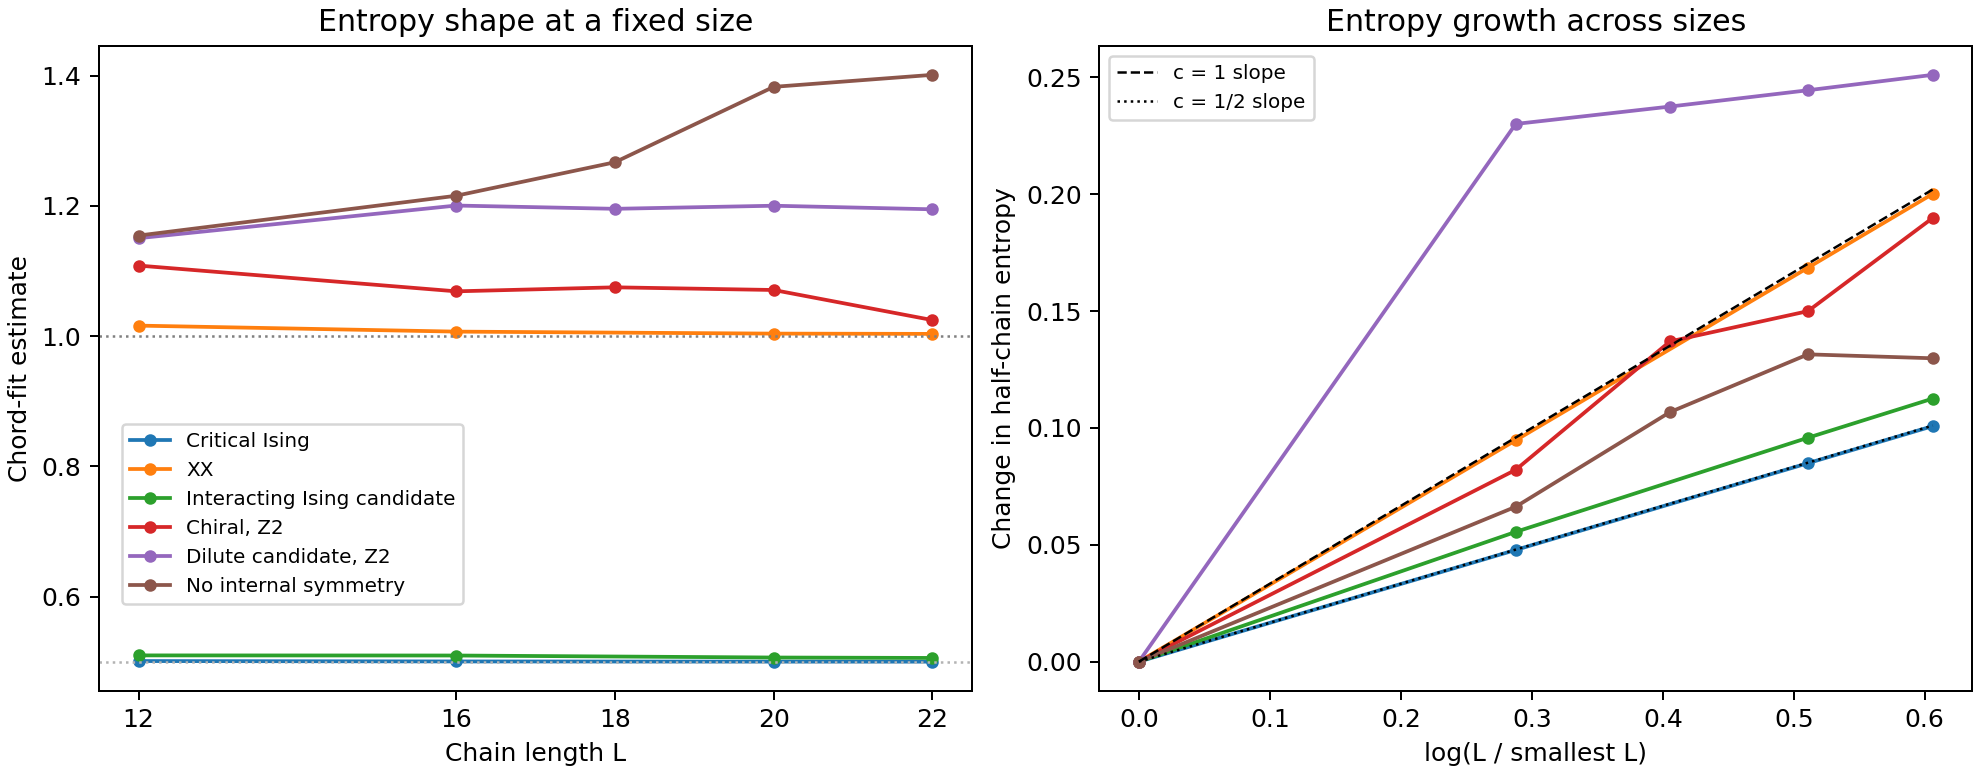
\includegraphics[width=\linewidth]{c6_entropy.png}
\caption{Fixed-size chord slopes and entropy growth across sizes. In the
right panel each curve is referenced to its smallest size. The high chord
slopes of the dilute and symmetry-free candidates do not agree with their
size growth. The exactly solved calibrations distinguish this failure from
an overall normalization error.}
\end{figure}

There are 108 all-momentum screening records and 710 stored multi-level
momentum/parity blocks in the main runs, in addition to tuning and crossing
calculations. The largest block has dimension 190746. The maximum stored
multi-level eigenvector residual is $1.08\times10^{-9}$. Residuals for
additional crossing calculations are stored separately. No sweep of the
full eight-parameter space, no thermodynamic extrapolation with controlled
errors, and no global exclusion of $c>1$ was performed.

\section{Tests that could decide a residual candidate}

The next useful search is a tuned search for critical surfaces, rather than
maximizing $c_{\rm chord}$ at one size. In the axial family one should vary
anisotropy, $J_z$, $D$, and field together, tracking both the Ising mass and
the putative second soft branch. At a candidate collision the distinction
between an additional linear mode and a vanishing velocity is decisive.
The free dispersion \eqref{eq:disp} supplies a benchmark where the latter
happens and the endpoint is not conformal.

For each candidate, the following tests are needed together.
\begin{enumerate}
\item Resolve every momentum and all exact internal sectors. Track the same
primary and descendant families as size changes, allowing moving Fermi
momenta and zero-mode changes. A putative Ising-times-boson theory should
have the Ising $1/8$ and 1 primaries and their descendants in addition to
Gaussian charge/winding and oscillator levels, with the appropriate
translation and symmetry selection rules. An alternative irreducible
$c>1$ theory needs its own consistent tower assignment.
\item Extract each chiral velocity from descendants and check it tends to
a nonzero value. Test $1/L$ against $1/L^2$ or other powers for the soft
branch. Fit the ground energy to the velocity-weighted Casimir expression
only after accounting for the identified zero modes. A new small gap alone
does not identify an additional CFT.
\item Require fixed-size entropy profiles and size-growth estimates to
agree above one over increasing size windows and away from isolated
sector crossings. Vary the short-distance cut exclusion. Ground-state
degeneracy and the choice of a superposition within it must be stated.
\item Use larger-system DMRG or uniform MPS, with converged bond dimensions,
as a follow-up to ED. Test finite-entanglement entropy versus correlation
length, conventionally $S\simeq(c/6)\log\xi$, while resolving distinct
correlation-length branches and checking for unit-cell or incommensurability
artifacts. That calculation was not run here.
\item In the symmetry-free family, tune the coefficient of every relevant
candidate CFT operator that is no longer forbidden, rather than assuming
that the Ising tuning survives symmetry breaking. Independently track
level crossings between the low-entropy and current-carrying branches.
\end{enumerate}
These tests could validate a counterexample at a specified point. Failure to
find one in a finite parameter search would still not prove the conjecture.

The analytic result is therefore a controlled union $\F\cup\U\cup\X$,
with the latter two components relying on stated exact-solution inputs, and
the algebraic residual set \eqref{eq:residual}. The numerical work gives a
consistent interacting Ising example and locates specific false-positive
or inconclusive entropy candidates. A theorem for the interacting residual
set, or a scale-consistent $c>1$ spectrum there, remains the missing result.

\appendix
\section{Reproduction}

All commands are run in the directory containing \texttt{c6.py}; outputs
append to \texttt{c6\_results.jsonl}. The summary deduplicates identical
model, size, and sector keys, keeps the last record, and excludes records
before the corrected code version. Representative commands are
\begin{verbatim}
python3 c6.py check
python3 c6.py run --model ising --lengths 12 16 20 22 --towers
python3 c6.py run --model xx --lengths 12 16 20 22 --towers
python3 c6.py tune --lengths 18 22 --D .1 --bracket 1.95 2.0
python3 c6.py run --model residual --field 1.9891 --D .1 \
  --lengths 12 16 20 22 --all-momenta
python3 c6.py sweep --lengths 12 16 --Ds .1 .2 .25 .3 .4 .6 \
  --fields 1.2 1.6 1.8 1.9 1.98 2.05
python3 c6.py run --model residual --field 2.05 --D .4 \
  --lengths 18 20 22 --all-momenta
python3 c6.py run --model residual --field 1.2 --D .4 \
  --lengths 18 20 22 --all-momenta
python3 c6.py sweep --model generic --lengths 12 16 \
  --Ds .1 .3 .4 --fields 1.2 1.9 1.98 2.05
python3 c6.py run --model generic --field 1.2 --D .4 \
  --lengths 18 20 22 --all-momenta
python3 c6.py run --model generic --field 1.2 --D .4 --tilt .5 \
  --lengths 16 20 22 --all-momenta --levels 2
python3 c6.py crossing --lengths 16 20 22 --bracket 1.0 1.3
python3 c6.py crossing-dispersion
python3 c6.py summarize
python3 c6.py plot
\end{verbatim}
The tilt commands are repeated for the values specified in the text.
\texttt{c6\_summary.json} and \texttt{c6\_tables.txt} contain the processed
numbers; the PNG and SVG entropy figures are standalone artifacts. The
LaTeX source is provided without a PDF compilation.
\end{document}
